
% Mikes: ok
% Spellcheck: ok

% ============================================================
\chapter{Intermezzo: A Data Analysis Session}{}{}
\label{ch:session}
  
\index{data analysis!session example|(}
   
\Fint{Occasionally I get the question: ``How do you actually work?''  or
``How do you come up with this} stuff?'' As an answer, I want to take
you on a tour through a new data set. I will use gnuplot, \index{plot function (gnuplot)} which is my
preferred tool for this kind of interactive data analysis---you will
see why. And I will share my observations and thoughts as we go along.

\section{A Data Analysis Session}
    
The data set is a classic: the $\mathrm{CO_2}$ measurements above
Mauna Loa on Hawaii. \index{CO2@$\mathrm{CO_2}$ measurements above Mauna Loa on Hawaii} The inspiration for this section comes from
Cleveland's \emph{Elements of Graphical Analysis},\footnote{\cit{The
    Elements of Graphing Data}{William S.\ Cleveland}{Hobart
    Press}{1994. The data itself (in a slightly different format) is
  available from StatLib:
  \url{http://lib.stat.cmu.edu/datasets/visualizing.data.zip} and from
  many other places around the Web}} but the approach is entirely
mine.
    
First question: what's in the data set? I see that the first column
represents the date (month and year) while the second contains the
measured $\mathrm{CO_2}$ concentration in parts per million. Here are
the first few lines:

\begin{verbatim}
Jan-1959        315.42
Feb-1959        316.32
Mar-1959        316.49
Apr-1959        317.56
...
\end{verbatim}

The measurements are regularly spaced (in fact, monthly), so I don't
need to parse the date in the first column; I simply\vadjust{\pagebreak} plot the second
column by itself. (In the figure, I have added tick labels on the
horizontal axis for clarity, but I am omitting the commands required
here---they are not essential.)

\begin{verbatim}
plot "data" u 1 w l
\end{verbatim}

The plot shows a rather regular short-term variation overlaid on a
nonlinear upward trend. (See Figure \ref{fig:session01}.)

\begin{figure}[t!]
  \centerline{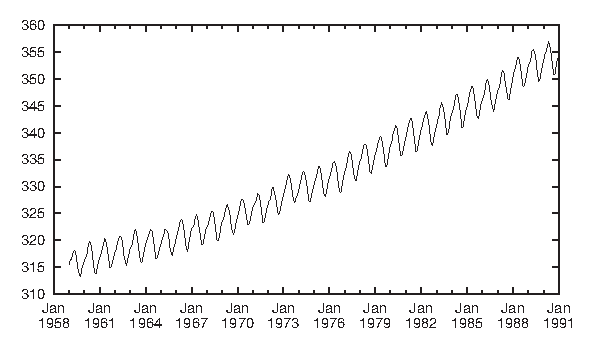
\includegraphics{img/session01}}
  \caption{The first look at the data: \hbox{\em plot ``data'' u 1 w l}}
  \label{fig:session01}
\end{figure}
    
The coordinate system is not convenient for mathematical modeling: the
$x$ axis is not numeric, and for modeling purposes it is usually helpful
if the graph goes through the origin. So, let's make it do so by
subtracting the vertical offset from the data and expressing the
horizontal position as the number of months since the first
measurement.  (This corresponds to the line number in the data file,
which is accessible in a gnuplot session through the pseudo-column
with column number 0.) 

\begin{verbatim}
plot "data" u 0:($2-315) w l
\end{verbatim}

A brief note on the command: the specification after the \texttt{u}
(short for \texttt{using}) gives the columns to be used for the $x$
and $y$ coordinates, separated by a colon. Here we use the line number
(which is in the pseudo-column 0) for the $x$ coordinate.  Also, we
subtract the constant offset 315 from the values in the second column
and use the result as the $y$ value. Finally, we plot the result
\texttt{with lines} (abbreviated \texttt{w l}) instead of using points
or other symbols. See Figure \ref{fig:session02}.

\begin{figure}[t!]
  \centerline{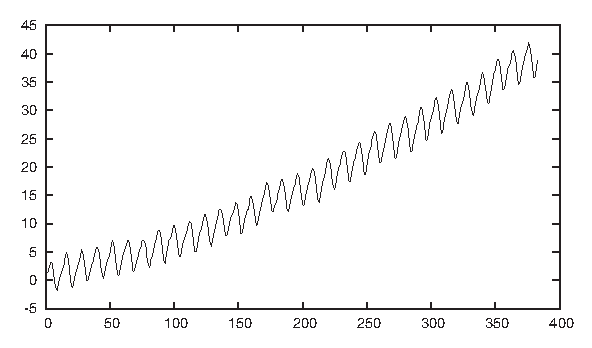
\includegraphics{img/session02}}
  \caption{Making the $x$ values numeric and subtracting the constant
    vertical offset: \hbox{\em plot ``data'' u 0:(\$2-315) w l}}
  \label{fig:session02}
\end{figure}
    
The most predominant feature is the trend. \index{trends!$\mathrm{CO_2}$ measurements above Mauna Loa on Hawaii} What can we say about it?
First of all, the trend is nonlinear: if we ignore the short-term
variation, the curve is convex downward. This suggests a power law
with an as-yet-unknown exponent: $x^k$. All power-law functions go
through the origin $(0,0)$ and also through the point $(1,1)$. We
already made sure that the data passes through the origin, but to fix
the upper-right corner, we need to rescale both axes: if $x^k$ goes
through $(1,1)$, then $b \paren{ \frac{x}{a} }^k$ goes through
$(a,b)$.
    
What's the value for the exponent $k$? All I know about it right now
is that it must be greater than 1 (because the function is convex).
Let's try $k=2$. (See Figure \ref{fig:session03}.)

\begin{verbatim}
plot "data" u 0:($2-315) w l, 35*(x/350)**2
\end{verbatim}

\begin{figure}[t!]
  \centerline{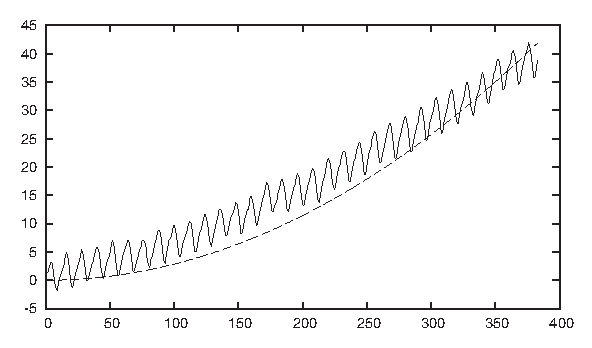
\includegraphics{img/session03}}
  \caption{Adding a function: \hbox{\em plot ``data'' u 0:(\$2-315) w l,
      35*(x/350)**2}}
  \label{fig:session03}
\end{figure}
    
Not bad at all! The exponent is a bit too large---some fiddling
suggests that $k=1.35$ would be a good value (see Figure
\ref{fig:session04}).

\begin{verbatim}
plot "data" u 0:($2-315) w l, 35*(x/350)**1.35
\end{verbatim}

\begin{figure}[t!]
  \centerline{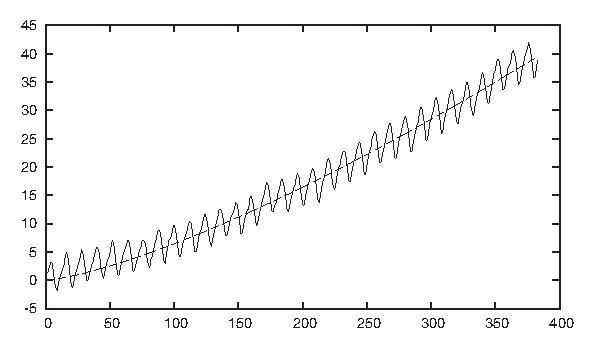
\includegraphics{img/session04}}
  \caption{Getting the exponent right: 
    $f(x) = 35 \paren{\frac{x}{350}}^{1.35}$}
  \label{fig:session04}
\end{figure}
    
To verify this, let's plot the residual; that is, we subtract the
trend from the data and plot what's left. If our guess for the trend
is correct, then the residual should not exhibit any trend itself---it
should just straddle $y=0$ in a balanced fashion (see Figure
\ref{fig:session05}).

\begin{verbatim}
plot "data" u 0:($2-315 - 35*($0/350)**1.35) w l
\end{verbatim}

\begin{figure}[t!]
  \centerline{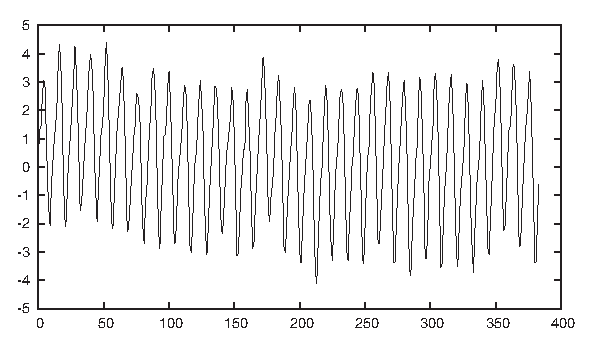
\includegraphics{img/session05}}
  \caption{The residual, after subtracting the function from the data.}
  \label{fig:session05}
\end{figure}
    
It might be hard to see the longer-term trend in this data, so we may
want to approximate it by a smoother curve. We can use the
weighted-spline approximation built into gnuplot for that purpose.  It
takes a third parameter, which is a measure for the smoothness: the
smaller the third parameter, the smoother the resulting curve; the
larger the third parameter, the more closely the spline follows the
original data (see Figure~\ref{fig:session06}).

\makeatletter
\def\texttt#1{{\fontsize{8}{10}\ttfamily\selectfont#1}}
\makeatother

\hspace*{18pt}\texttt{plot "data" u 0:($2-315 - 35*($0/350)**1.35) w l,
$\backslash$}\vspace*{-4pt}
\begin{verbatim}
     "" u 0:($2-315 - 35*($0/350)**1.35):(0.001) s acs w l
\end{verbatim}

\makeatletter
\def\texttt#1{{\fontsize{8.5}{10}\ttfamily\selectfont#1}}
\makeatother
    
At this point, the expression for the function that we use to
approximate the data has become unwieldy. Thus it now makes sense to
define it as a separate function:

\begin{verbatim}
f(x) = 315 + 35*(x/350)**1.35
plot "data" u 0:($2-f($0)) w l, "" u 0:($2-f($0)):(0.001) s acs w l
\end{verbatim}

\begin{figure}[t!]
  \centerline{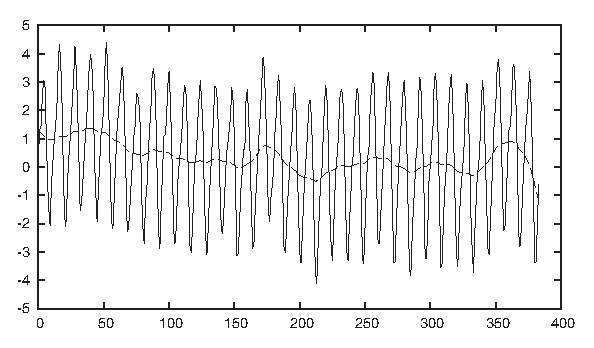
\includegraphics{img/session06}}
  \caption{Plotting a smoothed version of the residual together with
    the unsmoothed residual to test whether there is any systematic
    trend remaining in the residual.}
  \label{fig:session06}
\end{figure}

From the smoothed line we can see that the overall residual is pretty
much flat and straddles zero. Apparently, we have captured the overall
trend quite well: there is little evidence of a systematic drift
remaining in the residuals.

With the trend taken care of, the next feature to tackle is the
seasonality. \index{seasonality!$\mathrm{CO_2}$ measurements above Mauna Loa on Hawaii} The seasonality seems to consist of rather regular
oscillations, so we should try some combination of sines and cosines.
The data pretty much starts out at $y=0$ for $x=0$, so we can try a
sine by itself. To make a guess for its wavelength, we recall that the
data is meteorological and has been taken on a monthly basis---perhaps
there is a year-over-year periodicity. This would imply that the data
is the same every $12$ data points. If so, then a full period of the
sine, which corresponds to $2\pi$, should equal a horizontal distance
of $12$ points. For the amplitude, the graph suggests a value close to
$3$ (see Figure \ref{fig:session07}).

\begin{verbatim}
plot "data" u 0:($2-f($0)) w l, 3*sin(2*pi*x/12) w l
\end{verbatim}

\begin{figure}[t!]
  \centerline{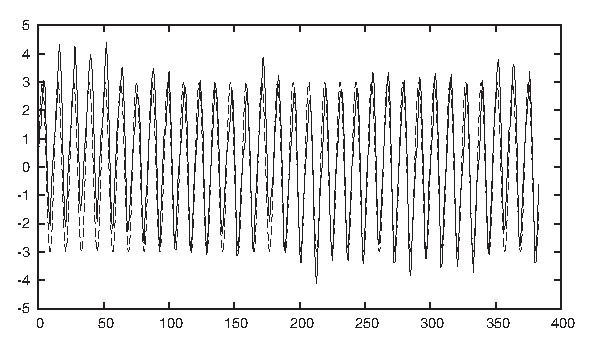
\includegraphics{img/session07}}
  \caption{Fitting the seasonality with a sine wave: 
    $3 \sin\paren{2\pi \frac{x}{12}}$}
  \label{fig:session07}\vspace*{-6pt}
\end{figure}
  
Right on! In particular, our guess for the wavelength worked out
really well. This makes sense, given the origin of the data.
    
Let's take residuals again, employing splines to see the bigger
picture as well (see Figure \ref{fig:session08}):

\begin{verbatim}
f(x) = 315 + 35*(x/350)**1.35 + 3*sin(2*pi*x/12)
plot "data" u 0:($2-f($0)) w l, "" u 0:($2-f($0)):(0.001) s acs w l
\end{verbatim}

\begin{figure}[t!]
  \centerline{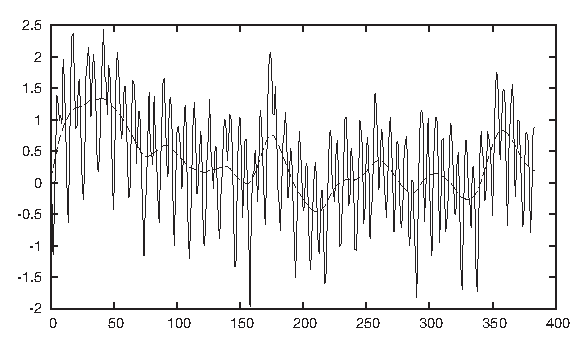
\includegraphics{img/session08}}
  \caption{Residuals after subtracting both trend and seasonality.}
  \label{fig:session08}\vspace*{-6pt}
\end{figure}
    
The result is pretty good but not good enough. There is clearly some
regularity remaining in the data, although at a higher frequency than
the main seasonality. Let's zoom in on a smaller interval of the data
to take a closer look. The data in the interval \texttt{[60:120]}
appears particularly regular, so let's look there (see Figure
\ref{fig:session09}):

\begin{verbatim}
plot [60:120] "data" u 0:($2-f($0)) w lp, "" u 0:($2-f($0)):(0.001) s acs w l
\end{verbatim}

\begin{figure}[t!]
  \centerline{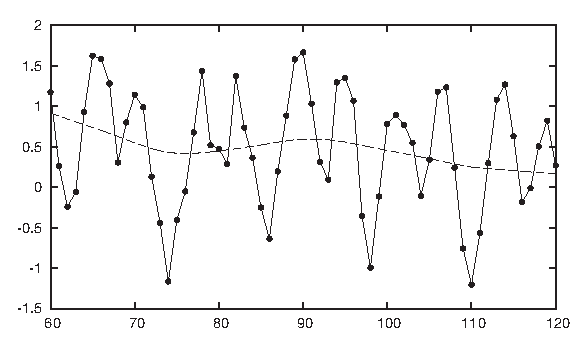
\includegraphics{img/session09}}
  \caption{Zooming in for a closer look. Individual data points are
    marked by symbols.}
  \label{fig:session09}
\end{figure}
    
I have indicated the individual data points using gnuplot's
\texttt{linespoints} (\texttt{lp}) style. We can now count the number
of data points between the main valleys in the data: $12$ points.
This is the main seasonality. But it seems that between any two
primary valleys there is exactly one secondary valley. Of course:
higher harmonics! The original seasonality had a period of exactly
$12$ months, but its shape was not entirely symmetric: its rising
flank comprised $7$ months but the falling flank only $5$ (as you can
see by zooming in on the original data with only the trend removed).
This kind of asymmetry implies that the seasonality cannot be
represented by a simple sine wave alone but that we have to take
into account higher harmonics---that is, sine functions with frequencies
that are integer multiples of the primary seasonality. So let's try
the first higher harmonic, again punting a little on the amplitude
(see Figure \ref{fig:session10}):

\begin{verbatim}
f(x) = 315 + 35*(x/350)**1.35 + 3*sin(2*pi*x/12) - 0.75*sin(2*pi*$0/6)
plot "data" u 0:($2-f($0)) w l, "" u 0:($2-f($0)):(0.001) s acs w l
\end{verbatim}

\begin{figure}[t!]
  \centerline{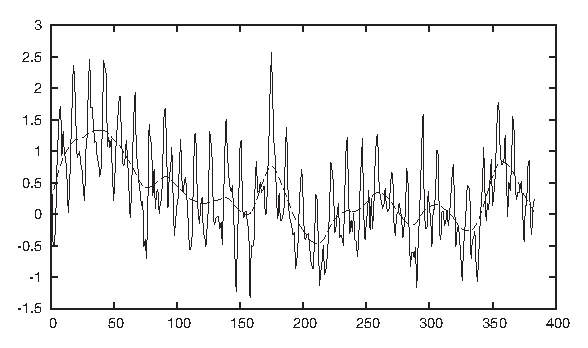
\includegraphics{img/session10}}
  \caption{Residual after removing trend and the first and second
    harmonic of the seasonality.}
  \label{fig:session10}
\end{figure}
    
Now we are really pretty close. Look at the residual---in particular,
for values of $x$ greater than about $150$. The data starts to look
quite ``random,'' although there is some systematic behavior for $x$
in the range \texttt{[0:70]} that we don't really capture. Let's add
some constant ranges to the plot for comparison (see Figure
\ref{fig:session11}):

\begin{verbatim}
plot "data" u 0:($2-f($0)) w l, "" u 0:($2-f($0)):(0.001) s acs w l, 0, 1, -1
\end{verbatim}
\begin{figure}[t!]
  \centerline{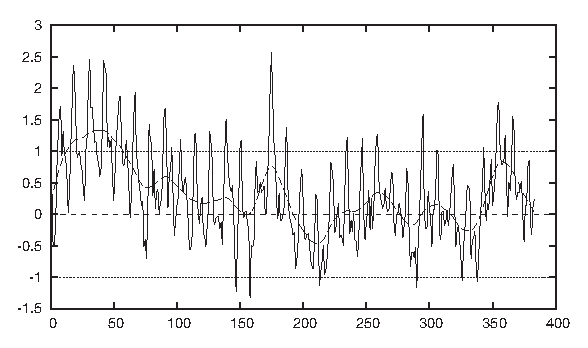
\includegraphics{img/session11}}
  \caption{Adding some grid lines for comparison.}
  \label{fig:session11}
\end{figure}
    
It looks as if the residual is skewed toward positive values, so let's
adjust the vertical offset by $0.1$ (see Figure \ref{fig:session12}):

\begin{verbatim}
f(x) = 315 + 35*(x/350)**1.35 + 3*sin(2*pi*x/12) - 0.75*sin(2*pi*$0/6) + 0.1
plot "data" u 0:($2-f($0)) w l, "" u 0:($2-f($0)):(0.001) s acs w l, 0, 1, -1
\end{verbatim}

\begin{figure}[t!]
  \centerline{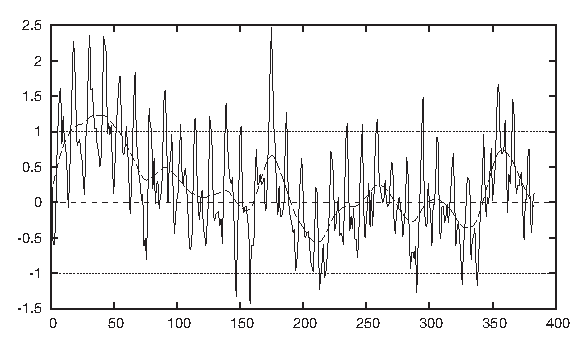
\includegraphics{img/session12}}
  \caption{The final residual.}
  \label{fig:session12}
\end{figure}
    
That's now really close. You should notice how small the last
adjustment was---we started out with data ranging from 300 to 350, and
now we are making adjustments to the parameters on the order of 0.1.
Also note how small the residual has become: mostly in the range from
$-0.7$ to $0.7$. That's only about 3 percent of the total variation in
the data.
    
Finally, let's look at the original data again, this time together
with our analytical model (see Figure \ref{fig:session13}):

\begin{verbatim}
f(x) = 315 + 35*(x/350)**1.35 + 3*sin(2*pi*x/12) - 0.75*sin(2*pi*$0/6) + 0.1
plot "data" u 0:2 w l, f(x)
\end{verbatim}

\begin{figure}[t!]
  \centerline{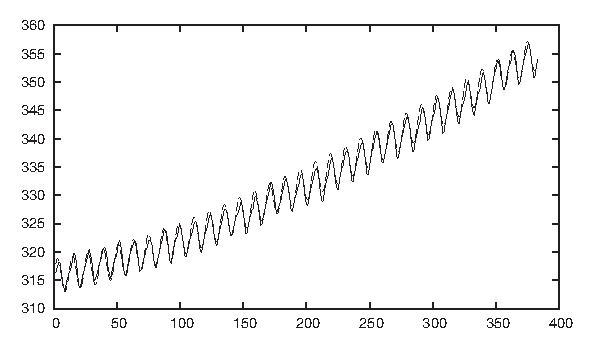
\includegraphics{img/session13}}
  \caption{The raw data with the final fit.}
  \label{fig:session13}
\end{figure}
    
All in all, pretty good.
    
So what is the point here? The point is that we started out with
nothing---no idea at all of what the data looked like. And then, layer
by layer, we peeled off components of the data, until only random
noise remained. We ended up with an explicit, analytical formula that
describes the data remarkably well.
    
But there is something more. We did so entirely ``manually'': by
plotting the data, trying out some approximations, and wiggling the
numbers until they agreed reasonably well with the data. At no point
did we resort to a black-box fitting routine---because we didn't have
to!  We did just fine. (In fact, after everything was finished, I tried
to perform a nonlinear fit using the functional form of the analytical
model as we have worked it out---only to have it explode terribly!
The model depends on seven parameters, which means that convergence of
a nonlinear fit can be a bit precarious.  In fact, it took me
\emph{longer} to try to make the fit work than it took me to work the
parameters out manually as just demonstrated.)
    
I'd go even further. We learned \emph{more} by doing this work
manually than if we had used a fitting routine. Some of the
observations (such as the idea to include higher harmonics) arose only
through direct interaction with the data. And it's not even true that
the parameters would be more accurate if they had been calculated by a
fitting routine.  Sure, they would contain 16 digits but not more
information. Our manual wiggling of the parameters enabled us to see
quickly and directly the point at which changes to the parameters are
so small that they no longer influence the agreement between the data
and the model.  That's when we have extracted all the information from
the data---any further ``precision'' in the parameters is just
insignificant noise.

\begin{figure}[t!]
  \centerline{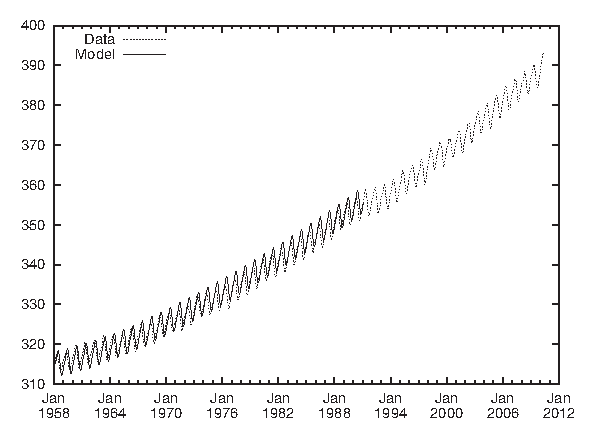
\includegraphics{img/session14}}
  \caption{The extended data set up to early 2010 together with the
    model (up to 1990).}
  \label{fig:session14}
\end{figure}

You might want to try your hand at this yourself and also experiment
with some variations of your own.  For example, you may question the
choice of the power-law behavior for the long-term trend.\vadjust{\pagebreak} 
Does an exponential function (like $\exp(x)$) give a better fit? It is not
easy to tell from the data, but it makes a huge difference if we want
to project our findings significantly (10 years or more) into the
future. You might also take a closer look at the seasonality. Because
it is so regular---and especially since its period is known
exactly---you should be able to isolate just the periodic part of the
data in a separate model by averaging corresponding months for all
years.  Finally, there is 20 years' worth of additional data available
beyond the ``classic'' data set used in my original
exploration.\footnote{You can obtain the data from the observatory's
  official website at
  \url{http://www.esrl.noaa.gov/gmd/}\url{ccgg/trends/}. Also check out the
  narrative (with photos of the apparatus!) at
  \url{http://celebrating200years.noaa.gov/datasets/mauna/welcome.html}.}
Figure \ref{fig:session14} shows all the available data together with
the model that we have developed. Does the fit continue to work well
for the years past 1990?

% ============================================================
\section{Workshop: gnuplot}

\index{gnuplot}

The example commands in this chapter should have given you a good idea
what working with gnuplot is like, but let's take a quick look at some
of the basics.

Gnuplot (\url{http://www.gnuplot.info}) is command-line oriented: when
you start gnuplot, it presents you with a text prompt at which to
enter commands; the resulting graphs are shown in a separate window.
Creating plots is simple---the command:

\begin{verbatim}
plot sin(x) with lines, cos(x) with linespoints
\end{verbatim}

will generate a plot of (you guessed it) a sine and a cosine. The
sine will be drawn with plain lines, and the cosine will be drawn
with symbols (``points'') connected by lines.

(Many gnuplot keywords can be abbreviated: instead of \texttt{with
  lines} I usually type: \texttt{w l}, or \texttt{w lp} instead of
\texttt{with linespoints}. These short forms are a major convenience
although rather cryptic in the beginning. In this short introductory
section, I will make sure to only use the full forms of all commands.)

To plot data from a file, you also use the \texttt{plot} command;
for instance:

\begin{verbatim}
plot "data" using 1:2 with lines
\end{verbatim}

When plotting data from a file, we use the \texttt{using} keyword to
specify which columns from the file we want to plot---in the command
just given, we use entries from the first column as $x$ values and use
entries from the second column for $y$ values.

One of the nice features of gnuplot is that you can apply arbitrary
transformations to the data as it is being plotted. To do so, you put
parentheses around each entry in the column specification that you
want to apply a transform to. Within these parentheses you can use any
mathematical expression. The data from each column is available by
prefixing the column index by the dollar sign. An example will make
this more clear:

\begin{verbatim}
plot "data" using (1/$1):($2+$3) with lines
\end{verbatim}

This command plots the sum of the second and third columns (that is:
\texttt{\$2+\$3}) as a function of one over the value in the first
column (\texttt{1/\$1}).

It is also possible to mix data and functions in a single plot command
(as we have seen in the examples in this chapter):

\begin{verbatim}
plot "data" using 1:2 with lines, cos(x) with lines
\end{verbatim}

This is different from the Matlab-style of plotting, where a function
must be explicitly \emph{evaluated} for a set of points before the
resulting set of values can be plotted.

We can now proceed to add decorations (such as labels and arrows) to
the plot. All kinds of options are available to customize virtually
every aspect of the plot's appearance: tick marks, the legend, aspect
ratio---you name it. When we are done with a plot, we can save all the
commands used to create it (including all decorations) via the
\texttt{save} command:

\begin{verbatim}
save "plot.gp"
\end{verbatim}

Now we can use \texttt{load "plot.gp"} to re-create the graph.

As you can see, gnuplot is extremely straightforward to use. The one
area that is often regarded as somewhat clumsy is the creation of
graphs in common graphics file formats. The reason for this is
historical: the first version of gnuplot was written in 1985, a time
when one could not expect every computer to be connected to a
graphics-capable terminal and when many of our current file formats
did not even exist!  The gnuplot designers dealt with this situation
by creating the so-called ``terminal'' abstraction. All
hardware-specific capabilities were encapsulated by this abstraction
so that the rest of gnuplot could be as portable as possible. Over
time, this ``terminal'' came to include different graphics \emph{file
  formats} as well (not just graphics hardware terminals), and this
usage continues to this day.

Exporting a graph to a common file format\index{files!formats}\index{exporting file formats from gnuplot} (such
as GIF, PNG, PostScript, or PDF) requires a five-step process:

\begin{verbatim}
set terminal png
set output "plot.png"
replot
set terminal wxt
set output
\end{verbatim}

In the first step, we choose the output device or ``terminal'': here,
a PNG file. In the second step, we choose the file name. In the third
step, we explicitly request that the graph be regenerated for this
newly chosen device. The remaining commands restore the interactive
session by selecting the interactive \texttt{wxt} terminal (built on
top of the wxWidgets widget set) and redirecting output back to the
interactive terminal. If you find this process clumsy and error-prone,
then you are not alone, but rest assured: gnuplot allows you to write
macros, which can reduce these five steps to one!

I should mention one further aspect of gnuplot: because it has been
around for 25 years, it is extremely mature and robust when it comes
to dealing with typical day-to-day problems. For example, gnuplot is
refreshingly unpicky when it comes to parsing input files. Many other
data analysis or plotting programs that I have seen are pretty rigid
in this regard and will bail when encountering unexpected data in an
input file. This is the right thing to do in theory, but in
practice, data files are often not clean---with ad hoc formats and
missing or corrupted data points. Having your plotting program balk
over whitespace instead of tabs is a \emph{major} nuisance when doing
real work. In contrast, gnuplot usually does an amazingly good job at
making sense of almost any input file you might throw at it, and that
is indeed a great help. Similarly, gnuplot recognizes undefined
mathematical expressions (such as $1/0$, $\log(0)$, and so on) and
discards them.  This is also very helpful, because it means that you
don't have to worry about the domains over which functions are
properly defined while you are in the thick of things. Because the
output is graphical, there is usually very little risk that this
silent discarding of undefined values will lead you to miss essential
behavior.  (Things are different in a computer program, where silently
ignoring error conditions usually only compounds the problem.)

% ============================================================
\section{Further Reading}

\begin{itemize}

\item \cit{Gnuplot in Action: Understanding Data with
    Graphs}{Philipp K.\ Janert}{Manning Publications}{2010}
  If you want to know more about gnuplot, then you may find this book
  interesting. It includes not only explanations of all sorts of
  advanced options, but also helpful hints for working with gnuplot.

\end{itemize}

\index{data analysis!session example|)}
